\documentclass[tikz,border=8pt]{standalone}
\usepackage[T1]{fontenc}
\usepackage{lmodern}
\usetikzlibrary{arrows.meta,positioning,fit,backgrounds}
\begin{document}
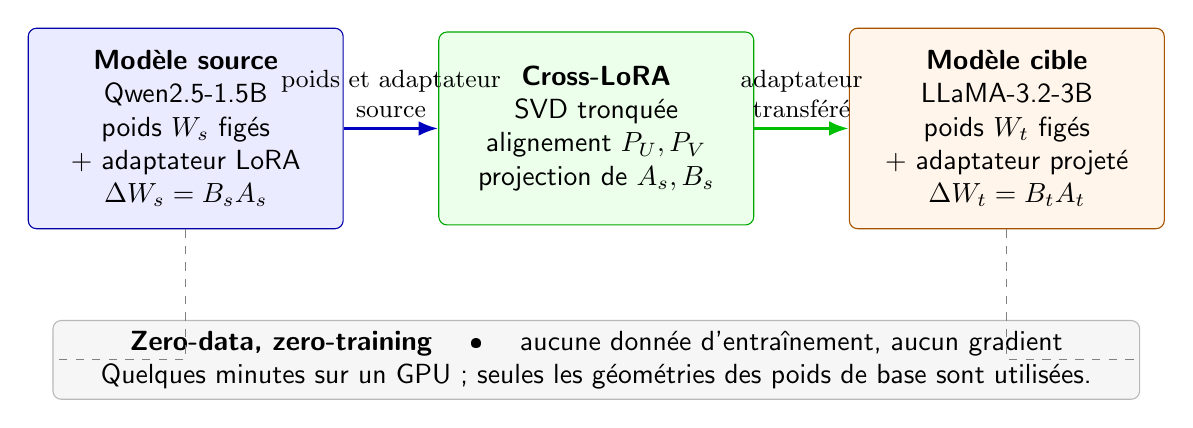
\begin{tikzpicture}[font=\sffamily, >=Latex, node distance=12mm,
 box/.style={draw=#1!65!black,fill=#1!8,rounded corners=3pt,align=center,minimum width=4.0cm,minimum height=2.45cm,inner sep=8pt},
 arrow/.style={-{Latex[length=2.5mm]},line width=1.1pt,draw=#1!75!black}]
\node[box=blue] (src) {\textbf{Modèle source}\\Qwen2.5-1.5B\\poids $W_s$ figés\\+ adaptateur LoRA\\$\Delta W_s=B_sA_s$};
\node[box=green,right=of src] (method) {\textbf{Cross-LoRA}\\SVD tronquée\\alignement $P_U,P_V$\\projection de $A_s,B_s$};
\node[box=orange,right=of method] (tgt) {\textbf{Modèle cible}\\LLaMA-3.2-3B\\poids $W_t$ figés\\+ adaptateur projeté\\$\Delta W_t=B_tA_t$};
\draw[arrow=blue] (src)--node[above,align=center,font=\small]{poids et adaptateur\\source} (method);
\draw[arrow=green] (method)--node[above,align=center,font=\small]{adaptateur\\transféré} (tgt);
\node[draw=gray!55,fill=gray!7,rounded corners=3pt,below=12mm of method,minimum width=13.8cm,minimum height=1.0cm,align=center] (note) {\textbf{Zero-data, zero-training} \quad • \quad aucune donnée d'entraînement, aucun gradient\\Quelques minutes sur un GPU ; seules les géométries des poids de base sont utilisées.};
\draw[dashed,gray] (src.south) |- (note.west);
\draw[dashed,gray] (tgt.south) |- (note.east);
\end{tikzpicture}
\end{document}
